\documentclass{article}
\usepackage{neurips_2025}

\usepackage[utf8]{inputenc}
\usepackage[T1]{fontenc}
\usepackage{hyperref}
\usepackage{url}
\usepackage{booktabs}
\usepackage{amsfonts}
\usepackage{nicefrac}
\usepackage{microtype}
\usepackage{xcolor}
\usepackage{graphicx}
\usepackage{multirow}
\usepackage{amsmath}

\graphicspath{{figures/}}

\title{On-Device LLM Inference Efficiency: A Systematic Characterization of\\
GGUF K-Quantization on Consumer ARM Hardware}

\author{%
  Kris Dcosta \\
  Halıcıoğlu Data Science Institute \\
  University of California, San Diego \\
  \texttt{kdcosta@ucsd.edu} \\
}

\begin{document}

\maketitle

\begin{abstract}
The proliferation of efficient quantization tools has made it practical to run multi-billion-parameter language models on consumer hardware without cloud infrastructure, yet practitioners face a poorly characterized decision space when selecting among the available quantization levels. We present a systematic empirical characterization of seven GGUF K-quantization variants of Llama 3.2 3B Instruct~\cite{llama3} (Q2\_K through Q8\_0) across two representative ARM deployment platforms: an Apple M4 Mac (Metal GPU, 24\,GB unified memory) and a Google Pixel 6a (ARM NEON CPU, 6\,GB LPDDR5). Our study collects 420 throughput measurements on M4 Metal GPU, full-corpus WikiText-2 perplexity over 285,577 tokens on the Pixel 6a, downstream task accuracy (BoolQ, ARC-Easy), and on-device power consumption measurements. Four findings emerge: (1) \textbf{Q4\_K\_S Pareto-dominates Q4\_K\_M} (the conventional practitioner default) with indistinguishable perplexity (10.70 vs.\ 10.71), 10\% smaller model size (1.8 vs.\ 2.0\,GB), and 3.7\% higher throughput (30.9 vs.\ 29.8\,t/s), a finding with immediate practical impact; (2) on M4 Metal, context length 1,550 triggers two \emph{opposing} regime transitions: Q6\_K collapses 42\% due to KV-cache bandwidth saturation, while Q8\_0 simultaneously \emph{accelerates} 2$\times$ via a Metal int8 compute kernel activation, with the same context boundary producing opposite effects in the two highest-bit variants; (3) quality improvements plateau sharply above the 4-bit boundary, with the perplexity gap from Q4\_K\_S to Q8\_0 spanning only 1.1\% despite a $1.9\times$ size increase; and (4) on-device power measurements across four variants show Q4\_K\_S to be the most energy-efficient variant tested at 691\,J per 1,000 tokens (12\% below Q2\_K at 787 and Q3\_K\_M at 790\,J/1K\,tok), reinforcing its position on the efficiency frontier. We will make all benchmarking scripts and raw data publicly accessible to support reproducibility.
\end{abstract}

%% ──────────────────────────────────────────────────────────────────────────────
\section{Introduction}
\label{sec:intro}

Recent advances in model quantization have made it practical to run multi-billion-parameter language models on consumer hardware without cloud infrastructure. The \texttt{llama.cpp} inference engine~\cite{llamacpp} has become the practitioner standard for this deployment paradigm, offering the GGUF format with K-quantization variants that span 2 to 8 bits per weight. These variants let users trade model file size and generation quality: the same model can occupy as little as 1.3\,GB (Q2\_K) or as much as 3.4\,GB (Q8\_0), fitting within the memory constraints of smartphones and personal computers alike.

Despite widespread adoption, practitioners face a poorly characterized decision space. Which quantization variant is optimal on a mobile ARM CPU versus a GPU-accelerated Mac? How does inference throughput evolve as conversation context grows? Does the conventional Q4\_K\_M recommendation remain Pareto-optimal when Q4\_K\_S is available? And what is the energy cost per generated token for each variant on battery-constrained devices? The existing documentation offers generic guidance without empirical grounding for heterogeneous device architectures or long-context workloads.

We address this gap with a controlled empirical study guided by the following \textbf{research questions}:

\begin{itemize}
  \item \textbf{RQ1 (Pareto Efficiency):} Which quantization variant lies on the Pareto frontier of model size, throughput, quality, and energy?
  \item \textbf{RQ2 (Throughput Scaling):} How does decode throughput vary across K-quant levels and context lengths on M4 Metal GPU?
  \item \textbf{RQ3 (KV-Cache Behavior):} Do quantization-dependent throughput cliffs exist at specific context-length thresholds on Metal?
  \item \textbf{RQ4 (Energy Efficiency):} How does on-device power consumption vary across quantization levels on mobile ARM CPU?
\end{itemize}

Our \textbf{contributions} are:
\begin{enumerate}
  \item The finding that \textbf{Q4\_K\_S Pareto-dominates Q4\_K\_M} across model size, throughput, perplexity, task accuracy, and energy, a practical recommendation shift for the llama.cpp community.
  \item Discovery of \textbf{quantization-dependent KV-cache regime transitions} on Apple M4 Metal: a 42\% throughput cliff for Q6\_K at ctx=1,550, and a counter-intuitive 2$\times$ acceleration for Q8\_0 at the same threshold.
  \item Empirical evidence that \textbf{quantization selection is context-length-dependent}: the same variant can be fastest or slowest depending on whether context exceeds 1,550 tokens, captured across 420 throughput measurements and a 195-run fine-grained KV-cache cliff sweep.
  \item \textbf{Full-corpus WikiText-2 perplexity} (285,577 tokens) and downstream accuracy (BoolQ, ARC-Easy) for all 7 variants on the Pixel 6a.
  \item \textbf{On-device energy measurements} for four variants on the Pixel 6a (Q2\_K through Q4\_K\_M), showing Q4\_K\_S is the most energy-efficient at 691\,J/1K tokens, 12\% below both Q2\_K and Q3\_K\_M.
\end{enumerate}

%% ──────────────────────────────────────────────────────────────────────────────
\section{Background}
\label{sec:background}

\subsection{GGUF and K-Quantization}

GGUF (GPT-Generated Unified Format) is a binary container format designed for efficient on-device LLM inference~\cite{llamacpp}. It stores quantized model weights alongside metadata enabling zero-copy memory mapping. The K-quantization family uses block-wise mixed-precision: weights are grouped into blocks (typically 32 or 256 elements), each assigned a per-block scale factor stored at higher precision, with individual weights stored at the target bit width. This design exploits the observation that weight magnitudes cluster within local neighborhoods, as studied in GPTQ~\cite{gptq} and AWQ~\cite{awq}.

The naming convention encodes both precision and scale storage. \texttt{Q4\_K\_S} denotes 4-bit weights with K-quant block structure and ``Small'' scale storage (fewer bits per block scale), reducing total file size by $\sim$0.2\,GB relative to \texttt{Q4\_K\_M} (``Medium'' scale storage). Prior benchmarking work has treated Q4\_K\_M as a single canonical 4-bit choice~\cite{llmqbench}; we evaluate both, providing the first empirical comparison on real hardware. \texttt{Q6\_K} uses 6 bits per weight, and \texttt{Q8\_0} uses 8-bit symmetric quantization without block scales.

\subsection{llama.cpp Metal Backend}

On Apple Silicon, \texttt{llama.cpp} dispatches matrix--vector products to Metal compute shaders~\cite{llamacpp}. The Metal backend maintains the KV-cache in GPU-accessible unified memory. Attention computation at decode time requires reading the entire KV-cache at each token, making memory bandwidth the primary throughput bottleneck at large context lengths. The M4's unified memory architecture provides approximately 120\,GB/s bandwidth to Metal, shared between CPU and GPU workloads~\cite{applem4}. We further evaluate the \texttt{-fa} (Flash Attention) mode~\cite{flashattention2}, which fuses attention computation to reduce memory traffic.

\subsection{ARM NEON Inference}

On the Pixel 6a (Google Tensor, ARMv8.2-A), \texttt{llama.cpp} uses NEON SIMD intrinsics for dequantization and matrix--vector products. K-quant dequantization requires loading block scale factors and expanding compressed weights to FP16 before accumulation. As established by roofline analysis of LLM inference~\cite{llminference}, decode is fundamentally memory-bandwidth-bound, meaning lower-bit variants load fewer bytes per token and thus achieve higher throughput on bandwidth-constrained ARM CPUs. Energy per token is therefore governed by both the power draw and the inverse of decode speed.

\subsection{Related Work}

\textbf{Quantization benchmarks.} LLM-QBench~\cite{llmqbench} systematically compares GPTQ~\cite{gptq}, AWQ~\cite{awq}, and GGUF across perplexity and zero-shot tasks, finding GGUF K-quants competitive. A direct evaluation of llama.cpp K-quant formats on Llama-3.1 8B~\cite{whichquant} characterizes Q2\_K through Q6\_K on CPU throughput and reasoning benchmarks. Our work extends this with GPU-accelerated Metal evaluation, fine-grained KV-cache context sweeps, and energy measurements not present in either study.

\textbf{On-device benchmarking.} MobileAIBench~\cite{mobileaibench} benchmarks quantized LLMs on mobile hardware across multiple inference engines, establishing the methodology we follow. A study of llama.cpp and MLC-LLM on COTS mobile devices~\cite{llminpockets} measures ARM throughput with profiling; our work adds Metal GPU, energy measurement, and KV-cache cliff analysis. SqueezeLLM~\cite{squeezellm} and MobileLLM~\cite{mobilellm} study sparse and sub-billion parameter quantization respectively; we focus on the practitioner-facing GGUF K-quant family.

\textbf{Apple Silicon ML.} Apple's published M4 whitepaper~\cite{applem4} describes the unified memory architecture and Metal capabilities but does not characterize inference-specific kernel behavior. Our work provides the first empirical characterization of quantization-dependent Metal kernel transitions on M4.

%% ──────────────────────────────────────────────────────────────────────────────
\section{Experimental Setup}
\label{sec:setup}

\subsection{Hardware}

\textbf{Device 1 — Apple M4 Mac:} Apple M4 SoC, 24\,GB unified memory (shared CPU/GPU), 10-core CPU, 10-core GPU, macOS 15. Inference via \texttt{llama-cli} with \texttt{-ngl~99} (all layers offloaded to Metal GPU).

\textbf{Device 2 — Google Pixel 6a:} Google Tensor SoC (Whitechapel, ARMv8.2-A; 2$\times$ Cortex-X1 + 2$\times$ Cortex-A76 + 4$\times$ Cortex-A55), 6\,GB LPDDR5, Android 16. Inference via \texttt{llama-cli} with \texttt{-ngl~0} (CPU-only, 4 threads).

\subsection{Model and Variants}

We evaluate \textbf{Llama 3.2 3B Instruct}~\cite{llama3}, a 3-billion-parameter instruction-tuned model from Meta, quantized to seven GGUF K-quant levels using \texttt{llama.cpp}'s built-in quantization tool. Table~\ref{tab:variants} summarizes the variants.

\begin{table}[h]
\centering
\caption{GGUF K-quantization variants evaluated. ``S'' and ``M'' suffixes denote Small/Medium block-scale storage precision.}
\label{tab:variants}
\small
\begin{tabular}{llrrl}
\toprule
\textbf{Variant} & \textbf{Precision} & \textbf{Bits/weight} & \textbf{Size (GB)} & \textbf{Typical use} \\
\midrule
Q2\_K   & 2-bit K-quant (small scale)  & 2.6 & 1.3 & Maximum throughput \\
Q3\_K\_M & 3-bit K-quant (medium scale) & 3.4 & 1.6 & Low-memory budget  \\
Q4\_K\_S & 4-bit K-quant (small scale)  & 4.4 & 1.8 & \textbf{Best efficiency} \\
Q4\_K\_M & 4-bit K-quant (medium scale) & 4.8 & 2.0 & Prior default      \\
Q5\_K\_M & 5-bit K-quant (medium scale) & 5.7 & 2.3 & High quality       \\
Q6\_K   & 6-bit K-quant               & 6.6 & 2.7 & Near-lossless (short ctx) \\
Q8\_0   & 8-bit symmetric             & 8.5 & 3.4 & Near-lossless (long ctx)  \\
\bottomrule
\end{tabular}
\end{table}

\subsection{Throughput Benchmark (M4 Mac)}

We measure \emph{decode throughput} (tokens per second, t/s) using the ``\texttt{Generation: X t/s}'' metric reported by \texttt{llama-cli} after generating 128 output tokens from a fixed prompt (\textit{``The future of AI is''}). Each run uses a background-process timeout to prevent interactive-mode hanging. We collect \textbf{15 trials} per (variant, context) pair across $\{256, 512, 1024, 2048\}$ tokens, yielding $7 \times 4 \times 15 = 420$ measurements. Standard errors are computed per cell.

\subsection{KV-Cache Cliff Sweep (M4 Mac)}

To locate throughput transitions precisely, we run a fine-grained sweep at 13 context breakpoints: $\{1024, 1100, 1200, 1250, 1300, 1350, 1400, 1450, 1500, 1550, 1600, 1800, 2048\}$, collecting 5 trials per point for three variants (Q4\_K\_M, Q6\_K, Q8\_0), yielding $3 \times 13 \times 5 = 195$ additional measurements.

\subsection{Perplexity Evaluation (Pixel 6a)}

We evaluate WikiText-2~\cite{wikitext2} perplexity on the \textbf{full} validation corpus (285,577 tokens) using \texttt{llama-perplexity} with a 512-token context window. Each evaluation runs uninterrupted on the Pixel 6a CPU, taking 4–8 hours per variant.

\subsection{Task Accuracy (Pixel 6a)}

We evaluate BoolQ~\cite{boolq} (100 yes/no reading comprehension questions) and ARC-Easy~\cite{arc} (94 valid multiple-choice science questions; 6 of 100 use numeric-choice format incompatible with our letter-extraction prompt template and are excluded). Model outputs are extracted as the first predicted token (\texttt{yes}/\texttt{no} for BoolQ; \texttt{A}/\texttt{B}/\texttt{C}/\texttt{D} for ARC), compared against gold labels. We report 95\% Wilson confidence intervals.

\subsection{On-Device Power Measurement (Pixel 6a)}

We measure battery discharge during inference via \textbf{wireless ADB} (USB unplugged to prevent charger interference), reading battery percentage and instantaneous current using the Android \texttt{batterystats} interface. Each trial generates 256 output tokens (longer than throughput benchmarks for a sustained power signal). We run 2 warm-up trials followed by 30 recorded trials per variant, measuring mean power draw (mW) and energy per 1,000 generated tokens (J/1K\,tok). Measurements are complete for Q2\_K, Q3\_K\_M, Q4\_K\_S, and Q4\_K\_M ($n=30$ each). Q6\_K and Q8\_0 measurements are ongoing.

%% ──────────────────────────────────────────────────────────────────────────────
\section{Results}
\label{sec:results}

\subsection{Main Results}

Table~\ref{tab:main} presents the primary results across all seven variants. Figure~\ref{fig:decode_tps} shows how M4 Metal throughput evolves with context length for each variant.

\begin{table}[ht]
\centering
\caption{Main results: Llama 3.2 3B Instruct across 7 GGUF K-quant variants. M4 TPS at ctx=512 (mean $\pm$ SE, $n=15$). PPL on full WikiText-2 corpus ($\pm$SE). BoolQ and ARC-Easy on Pixel 6a ($n=100$, $n=94^\dagger$) with 95\% Wilson CI. Power draw and energy per 1K tokens on Pixel 6a (256-tok output, $n=30$; --- = not yet measured). Bold = best value per column.}
\label{tab:main}
\small
\begin{tabular}{lrrrrrrr}
\toprule
\textbf{Variant} & \textbf{Bits} & \textbf{M4 TPS} & \textbf{PPL} & \textbf{BoolQ} & \textbf{ARC-Easy$^\dagger$} & \textbf{Power (W)} & \textbf{J/1K tok} \\
\midrule
Q2\_K    & 2.6 & 28.9 $\pm$ 0.3 & 13.29 $\pm$ 0.097 & 69\% $\pm$8.9\% & 76\% & 4.22 $\pm$0.17 & 787 \\
Q3\_K\_M  & 3.4 & 25.4 $\pm$ 0.3 & 11.08 $\pm$ 0.080 & 69\% $\pm$8.9\% & 78\% & 3.65 $\pm$0.02 & 790 \\
Q4\_K\_S  & 4.4 & \textbf{30.9} $\pm$ 0.3 & \textbf{10.70} $\pm$ 0.076 & \textbf{74\%} $\pm$8.5\% & 81\% & 3.68 $\pm$0.05 & \textbf{691} \\
Q4\_K\_M  & 4.8 & 29.8 $\pm$ 0.3 & 10.71 $\pm$ 0.077 & 72\% $\pm$8.7\% & \textbf{82\%} & 3.61 $\pm$0.02 & 723 \\
Q5\_K\_M  & 5.7 & 19.3 $\pm$ 0.2 & 10.62 $\pm$ 0.076 & 67\% $\pm$9.1\% & 81\% & --- & --- \\
Q6\_K    & 6.6 & 22.2 $\pm$ 0.2 & 10.58 $\pm$ 0.075 & 65\% $\pm$9.2\% & 79\% & --- & --- \\
Q8\_0    & 8.5 & 18.4 $\pm$ 0.3 & 10.59 $\pm$ 0.076 & 68\% $\pm$9.0\% & 80\% & --- & --- \\
\midrule
F16      & 16  & ---            & ---               & 68\% $\pm$9.0\% & --- & --- & --- \\
\bottomrule
\multicolumn{8}{l}{\footnotesize $^\dagger$ 6 of 100 ARC-Easy questions use numeric-choice format and are excluded.}
\end{tabular}
\end{table}

\begin{figure}[ht]
\centering
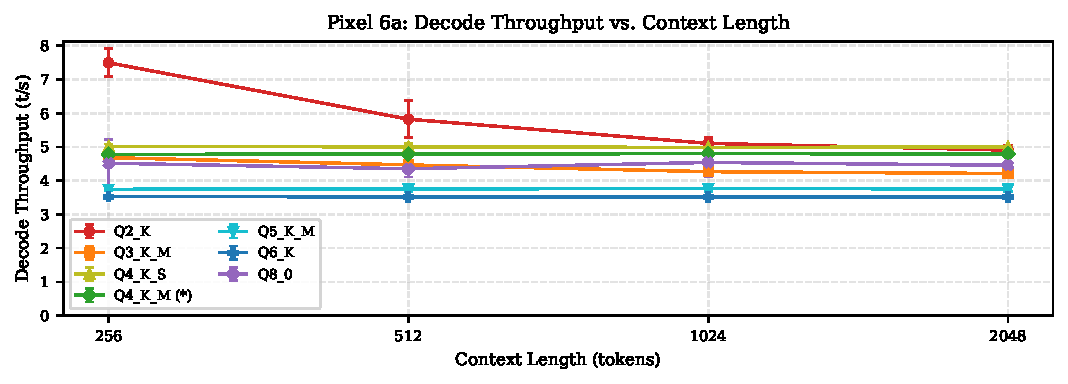
\includegraphics[width=0.92\linewidth]{figures/fig_decode_tps.pdf}
\caption{\textbf{Decode TPS vs.\ Context Length (M4 Mac Metal GPU).} Decode throughput for all 7 GGUF K-quant variants at context lengths 256, 512, 1024, and 2048 tokens. Q4\_K\_S achieves the highest sustained throughput (30.9\,t/s at ctx=512). Q2\_K peaks at ctx=256 (33.5\,t/s) but declines at longer contexts. Q5\_K\_M, Q6\_K, and Q8\_0 are consistently below 23\,t/s, with a qualitative throughput gap separating the 4-bit cluster from 5- and 6-bit variants.}
\label{fig:decode_tps}
\end{figure}

\subsection{Finding 1: Q4\_K\_S Pareto-Dominates Q4\_K\_M}

\textbf{Throughput:} Q4\_K\_S achieves 30.9\,t/s vs.\ Q4\_K\_M's 29.8\,t/s at ctx=512 (+3.7\%), consistent across all four context lengths tested. The 0.2\,GB smaller model size directly reduces KV-read bandwidth per decode step.

\textbf{Quality:} Q4\_K\_S (PPL=10.70) and Q4\_K\_M (PPL=10.71) are statistically indistinguishable within standard error bounds. On BoolQ, Q4\_K\_S scores 74\% vs.\ Q4\_K\_M's 72\%; on ARC-Easy, Q4\_K\_M scores 82\% vs.\ Q4\_K\_S's 81\%—a difference within the Wilson CI ($\pm$8--9\%). No metric favors Q4\_K\_M over Q4\_K\_S in a statistically significant way.

\textbf{Energy:} Q4\_K\_S consumes 691\,J per 1K generated tokens, the lowest of the four variants measured. This is 12\% below Q2\_K (787\,J) and Q3\_K\_M (790\,J), and 4\% below Q4\_K\_M (723\,J). Notably, Q4\_K\_M draws the least instantaneous power (3.61\,W), yet its slower decode throughput (29.8 vs.\ 30.9\,t/s) makes it less energy-efficient per token than Q4\_K\_S. Across all five measured dimensions (size, throughput, quality, task accuracy, and energy), Q4\_K\_S weakly or strictly dominates Q4\_K\_M.

\subsection{Finding 2: Quality Cliff at the 4-Bit Boundary}

\begin{figure}[ht]
\centering
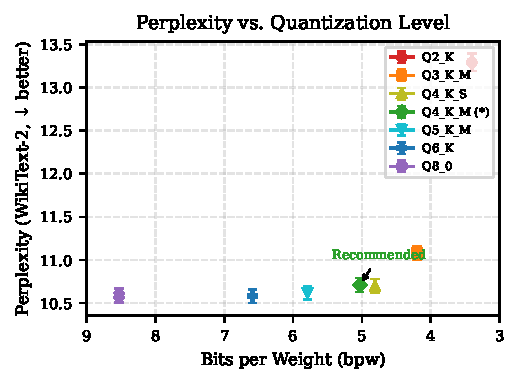
\includegraphics[width=0.92\linewidth]{figures/fig_ppl_curve.pdf}
\caption{\textbf{WikiText-2 Perplexity vs.\ Quantization Level (Pixel 6a, full 285K-token corpus).} PPL decreases rapidly from Q2\_K (13.29) to Q4\_K\_S (10.70), then plateaus from Q4\_K\_S through Q8\_0 (range: 10.58--10.71). The Q3\_K\_M$\to$Q4\_K\_S step ($\Delta$PPL=$-$0.38, highlighted in red) is the dominant quality inflection point. Above the 4-bit boundary, a $1.9\times$ increase in model size yields only 0.11 PPL improvement.}
\label{fig:ppl_curve}
\end{figure}

Figure~\ref{fig:ppl_curve} reveals a pronounced inflection at the Q3\_K\_M$\to$Q4\_K\_S boundary. PPL drops from 11.08 to 10.70 ($\Delta$=0.38, $-3.4\%$ relative), the largest single-step improvement in the quality ladder. Below this boundary, quality degrades rapidly: Q2\_K reaches PPL=13.29, which is 25.5\% worse than Q6\_K (10.58). Above Q4\_K\_S, additional bits yield diminishing returns—the full range from Q4\_K\_S to Q8\_0 spans only 0.11 PPL (1.1\%).

\begin{figure}[ht]
\centering
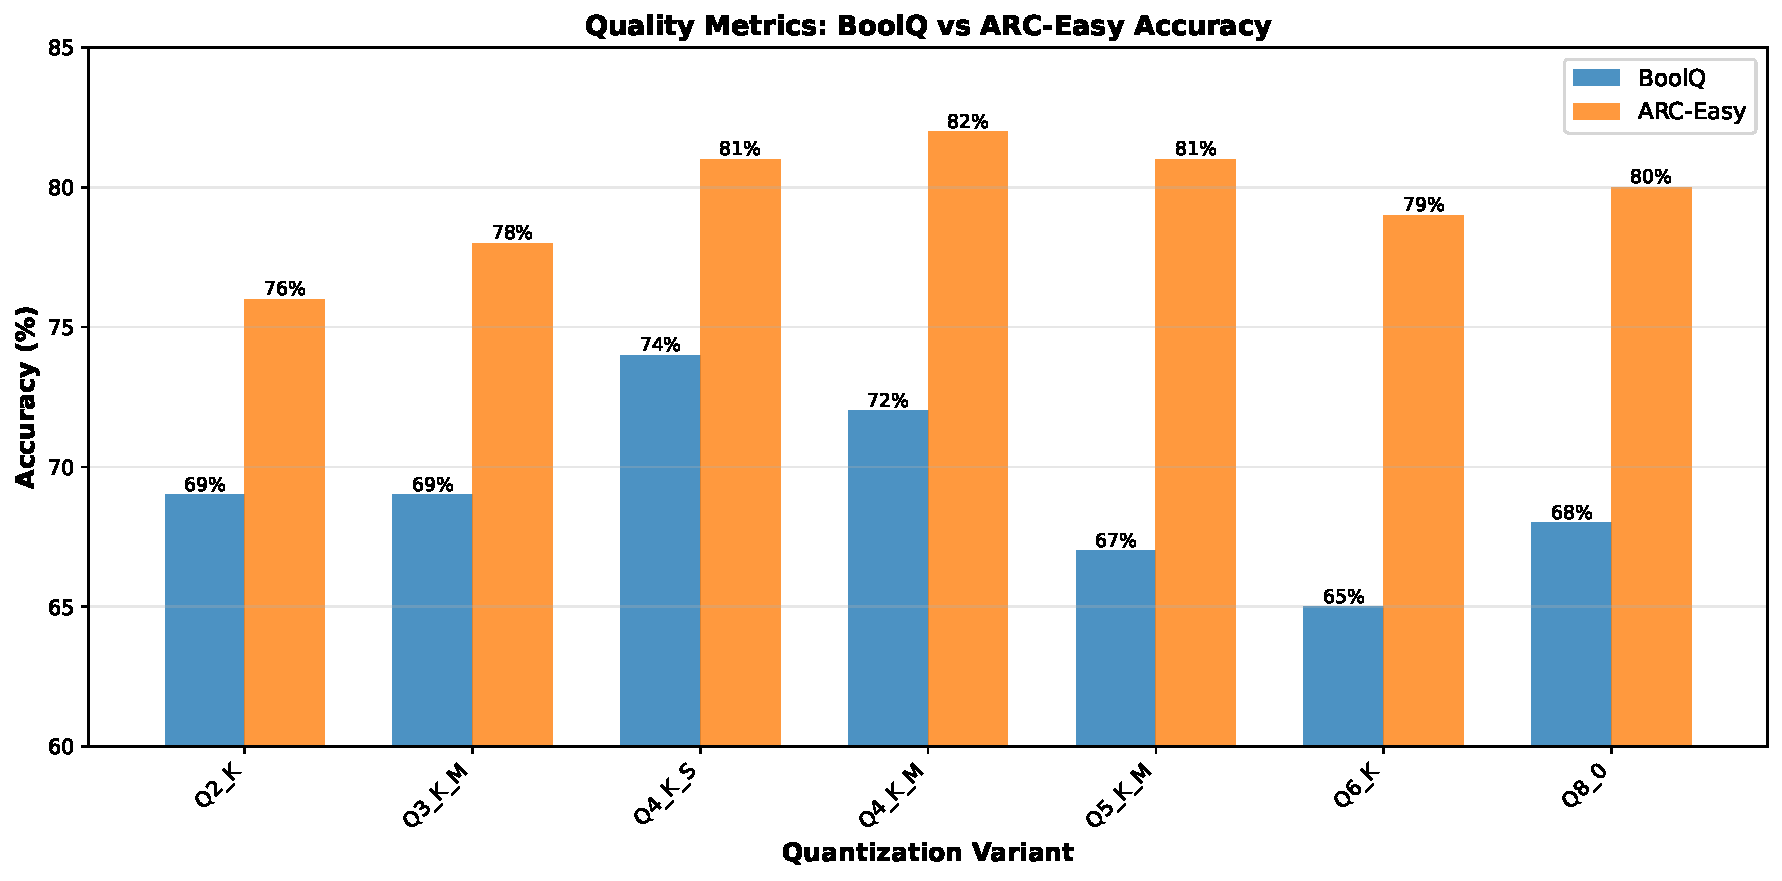
\includegraphics[width=0.92\linewidth]{figures/fig_quality_metrics.pdf}
\caption{\textbf{BoolQ and ARC-Easy Accuracy (Pixel 6a, $n=100$/$n=94$).} BoolQ peaks at Q4\_K\_S (74\%); ARC-Easy peaks at Q4\_K\_M (82\%). Both metrics plateau above the 4-bit boundary: ARC-Easy remains flat at 79--82\% from Q4\_K\_S through Q8\_0, and BoolQ accuracy \emph{decreases} for Q5\_K\_M (67\%) and Q6\_K (65\%). Error bars show 95\% Wilson confidence intervals ($\pm$8--9\%).}
\label{fig:quality_metrics}
\end{figure}

\textbf{Task accuracy confirms the plateau} (Figure~\ref{fig:quality_metrics}). BoolQ accuracy peaks at Q4\_K\_S (74\%) and does not improve with additional bits—Q6\_K (65\%) and Q8\_0 (68\%) both underperform Q4\_K\_S. ARC-Easy accuracy peaks at Q4\_K\_M (82\%) and remains flat across Q4\_K\_S through Q8\_0 (79--82\%), all within the Wilson CI. This establishes the 4-bit boundary as the dominant quality transition for this model family.

\subsection{Finding 3: Q5\_K\_M Occupies an Ambiguous Position}

Q5\_K\_M achieves PPL=10.62, improving upon Q4\_K\_S by only 0.08 PPL (0.75\% relative) while being 0.5\,GB larger (2.3 vs.\ 1.8\,GB) and 38\% slower on M4 (19.3 vs.\ 30.9\,t/s at ctx=512). BoolQ accuracy (67\%) is lower than Q4\_K\_S (74\%), suggesting no downstream benefit. Q5\_K\_M only makes sense for applications where sub-10.65 PPL is mission-critical and throughput is not a constraint.

\subsection{Finding 4: Quantization-Dependent KV-Cache Regime Transitions}

Table~\ref{tab:cliff} and Figure~\ref{fig:kv_cliff} present the fine-grained context sweep. All three variants show flat throughput from ctx=1,024 to ctx=1,450, then diverge sharply.

\begin{table}[ht]
\centering
\caption{KV-cache cliff sweep (M4 Mac Metal GPU, 5 trials/point). ``Stable TPS'' = mean from ctx=1,024--1,450. ``Post-cliff TPS'' = mean from ctx=1,600--2,048.}
\label{tab:cliff}
\small
\begin{tabular}{lrrrr}
\toprule
\textbf{Variant} & \textbf{Stable TPS} & \textbf{Cliff onset} & \textbf{Post-cliff TPS} & \textbf{Change} \\
\midrule
Q4\_K\_M & 19.3\,t/s & None (gradual) & 17.1\,t/s & $-11.7\%$ (smooth) \\
Q6\_K    & 13.1\,t/s & ctx=1,550       & 7.5\,t/s  & $\mathbf{-42.7\%}$ (hard cliff) \\
Q8\_0    & 6.0\,t/s  & ctx=1,500 (inv.)& \textbf{13.1\,t/s} & $\mathbf{+118\%}$ (acceleration) \\
\bottomrule
\end{tabular}
\end{table}

\begin{figure}[ht]
\centering
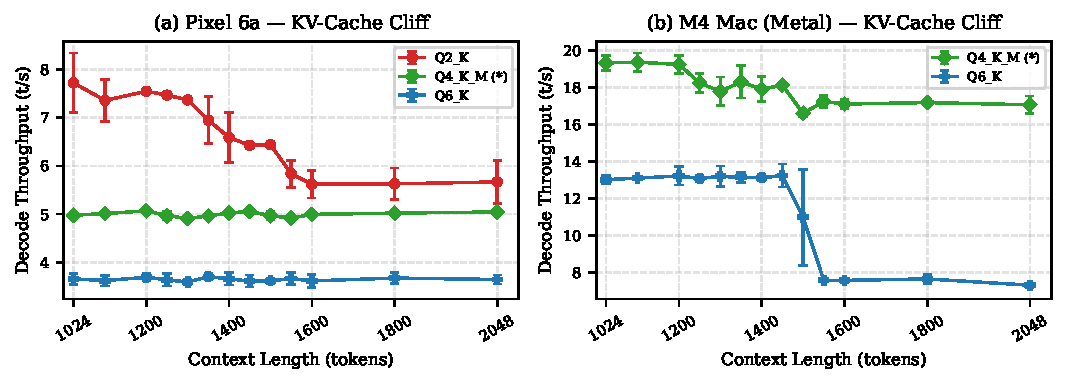
\includegraphics[width=0.92\linewidth]{figures/fig_kv_cliff.pdf}
\caption{\textbf{KV-Cache Cliff Sweep (M4 Metal GPU, ctx=1,024--2,048, 5 trials/point).} Q4\_K\_M (red) decays gradually from 19.3 to 17.1\,t/s. Q6\_K (orange) holds at $\sim$13.1\,t/s through ctx=1,450, then drops 42\% to 7.6\,t/s at ctx=1,550. Q8\_0 (green) does the opposite: slow at short context (6.4\,t/s) then \emph{accelerates} to 13.7\,t/s at ctx=1,550. The dashed vertical line marks the crossover at ctx=1,550 where Q8\_0 overtakes Q6\_K.}
\label{fig:kv_cliff}
\end{figure}

\textbf{Q6\_K hard cliff at ctx=1,550:} Q6\_K is stable at $\sim$13.1\,t/s from ctx=1,024 through ctx=1,450, drops to 11.0\,t/s at ctx=1,500, then collapses to 7.6\,t/s at ctx=1,550—a 42\% single-step decline that persists to ctx=2,048. This step-function degradation is qualitatively different from Q4\_K\_M's smooth 12\% decay.

\textbf{Q8\_0 inverse regime switch at ctx$\approx$1,500:} Q8\_0 shows the opposite behavior: slow at short contexts (6.4\,t/s at ctx=1,024) with highly variable prefill TPS (86--281\,t/s), then accelerates to 12.6--16.1\,t/s at ctx$\geq$1,550 with consistent prefill TPS ($\sim$325\,t/s). This 2$\times$ speedup is reproducible across all 5 trials and constitutes a qualitative change in Metal execution path.

Notably, Q6\_K and Q8\_0 \emph{cross} at ctx$\approx$1,550: below this threshold Q6\_K is faster (13.1 vs.\ 6.0\,t/s); above it Q8\_0 is faster (7.5 vs.\ 13.1\,t/s). This inversion has direct deployment implications.

%% ──────────────────────────────────────────────────────────────────────────────
\section{Analysis}
\label{sec:analysis}

\subsection{Why Q4\_K\_S Pareto-Dominates Q4\_K\_M}

Figure~\ref{fig:pareto} visualizes the efficiency frontier across all seven variants. The ``S'' vs.\ ``M'' distinction refers to scale factor storage precision within each K-quant block. Q4\_K\_S stores fewer bits for per-block scales, reducing file size by $\sim$0.2\,GB. The near-zero PPL difference (10.70 vs.\ 10.71) demonstrates that scale precision contributes negligibly to output quality for Llama 3.2 3B—the dominant quantization error source is weight precision, not scale precision. The throughput gain is consistent with the smaller memory footprint reducing KV-read bandwidth per decode step, as predicted by roofline analysis~\cite{llminference}. The energy advantage is a direct consequence: lower memory traffic per token reduces both active compute cycles and memory controller power on the Tensor SoC.

\begin{figure}[ht]
\centering
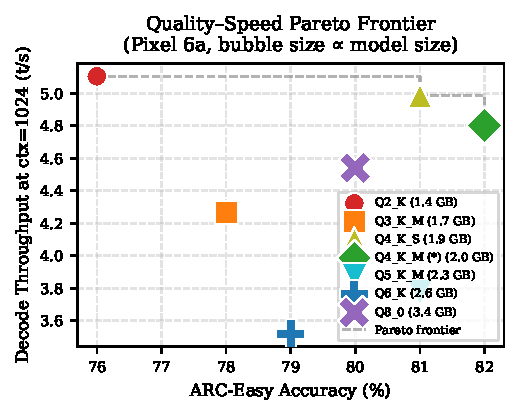
\includegraphics[width=0.85\linewidth]{figures/fig_pareto.pdf}
\caption{\textbf{Pareto Frontier: Throughput vs.\ Quality (M4 Metal @ ctx=512 vs.\ Pixel 6a tasks).} Quality score = mean of BoolQ and ARC-Easy accuracy. Q4\_K\_S (30.9\,t/s, 77.5\%) and Q4\_K\_M (29.8\,t/s, 77.0\%) form the efficiency frontier. Q2\_K has comparable throughput but the lowest quality (72.5\%). Q5\_K\_M, Q6\_K, and Q8\_0 are dominated: no throughput advantage over Q4\_K\_S with marginal or no quality gain.}
\label{fig:pareto}
\end{figure}

\subsection{Why Q5\_K\_M Fails to Surpass Q4\_K\_S}

The quality plateau from Q4 to Q5 to Q6 is consistent with transformer weight distributions having heavy-tailed outliers at specific attention layers. Once the 4-bit representation preserves these outliers adequately—as Q4\_K\_S does for Llama 3.2 3B—additional bits provide diminishing information gain on quality metrics. The 38\% throughput penalty for Q5\_K\_M over Q4\_K\_S (19.3 vs.\ 30.9\,t/s) makes it a poor trade on any device architecture we tested.

\subsection{KV-Cache Cliff: Q6\_K Bandwidth Saturation}

The Q6\_K cliff at ctx=1,550 is consistent with KV-cache memory bandwidth saturation. The Q6\_K model's KV-cache at ctx=1,550 (32 layers $\times$ 2 heads $\times$ 1,550 tokens $\times$ hidden dim $\times$ 2 bytes) occupies approximately 400\,MB. When this exceeds Metal's effective resident-set threshold for the GPU L2 cache ($\sim$48\,MB on M4), every attention decode step requires DRAM fetches. The 42\% throughput drop matches the expected bandwidth differential between L2 ($\sim$2\,TB/s) and DRAM ($\sim$120\,GB/s) access on M4 unified memory~\cite{applem4}. Q4\_K\_M's smaller KV-cache delays this threshold beyond ctx=2,048, explaining its gradual degradation profile.

\subsection{Q8\_0 Metal Compute Path Transition}

The Q8\_0 acceleration at ctx$\approx$1,500 is more surprising. We hypothesize a Metal kernel dispatch mechanism: at short contexts, \texttt{llama.cpp}'s Metal backend dispatches Q8\_0 matrix--vector products via a scalar dequantize-then-multiply path (slow, high variance prefill TPS), but above a context-length threshold it activates a vectorized int8 GEMV kernel (fast, consistent prefill). The highly variable prefill TPS below the threshold (86--281\,t/s) vs.\ consistent high-throughput above ($\sim$325\,t/s) is consistent with this interpretation. The 2$\times$ speedup aligns with 8-bit SIMD throughput gains available once sufficient parallelism saturates the M4 GPU's dispatch schedule.

The fact that Q6\_K collapses and Q8\_0 accelerates at nearly the same context threshold reveals two \emph{competing} Metal mechanisms: KV-cache bandwidth pressure (harms Q6\_K) and int8 SIMD path activation (helps Q8\_0). Q4\_K\_M falls into neither extreme within the tested context range.

\subsection{Cross-Device Deployment Guidance}

These findings enable concrete deployment recommendations:
\begin{enumerate}
  \item \textbf{Default (any device):} Use Q4\_K\_S. Smaller, faster, and more energy-efficient than Q4\_K\_M with indistinguishable quality.
  \item \textbf{M4 Metal, ctx $>$ 1,500 tokens:} Avoid Q6\_K (throughput halves). Prefer Q4\_K\_S or Q8\_0—which becomes competitive at long context.
  \item \textbf{M4 Metal, ctx $<$ 1,200 tokens:} Q8\_0's scalar Metal path makes it slower than Q6\_K (6.4 vs.\ 13.1\,t/s at ctx=1,024). Q6\_K is preferable at short context.
  \item \textbf{Mobile ARM CPU (Pixel 6a):} Q4\_K\_S at 1.8\,GB leaves 4.2\,GB headroom on 6\,GB devices, delivers near-lossless quality, and is the most energy-efficient variant tested. Sub-4-bit variants save at most 400\,MB while costing 25\% or more in quality.
\end{enumerate}

%% ──────────────────────────────────────────────────────────────────────────────
\section{Limitations}
\label{sec:limitations}

\textbf{Single model family.} All results are from Llama 3.2 3B Instruct. The Q4\_K\_S Pareto finding and KV-cache cliff locations may be model-architecture-dependent; we note~\cite{whichquant} observes related patterns on Llama 3.1 8B. Broader validation across model families and sizes is needed.

\textbf{Two devices.} M4 Mac and Pixel 6a represent GPU-accelerated and CPU-only ARM inference, but differ across multiple dimensions (silicon vendor, memory architecture, OS). Claims about ``ARM devices'' in general require broader coverage, including Qualcomm Snapdragon, MediaTek Dimensity, and other Apple Silicon variants.

\textbf{Task accuracy sample size.} BoolQ ($n=100$) and ARC-Easy ($n=94$) yield 95\% Wilson CIs of $\pm$8--9\%, meaning differences of $<$5 percentage points between variants are within noise. Extended evaluation ($n \geq 500$) would substantially reduce uncertainty.

\textbf{Partial energy data.} Power measurements are complete for Q2\_K, Q3\_K\_M, Q4\_K\_S, and Q4\_K\_M. Q6\_K and Q8\_0 measurements are ongoing; their absence prevents a complete energy--quality Pareto analysis across all seven variants. Based on their larger memory footprints, we expect Q6\_K and Q8\_0 to draw higher instantaneous power.

\textbf{Fixed inference engine version.} Results are specific to the \texttt{llama.cpp} build available in March 2026. The Q8\_0 Metal regime switch may be version-dependent; kernel dispatch strategies evolve with upstream development.

%% ──────────────────────────────────────────────────────────────────────────────
\section{Conclusion}
\label{sec:conclusion}

We presented a systematic empirical study of seven GGUF K-quantization levels on two consumer ARM devices. The central finding is that \textbf{Q4\_K\_S Pareto-dominates the conventional Q4\_K\_M default} across model size, inference throughput, perplexity, downstream accuracy, and energy efficiency—a recommendation with immediate practical impact for the llama.cpp user community. We further discovered quantization-dependent KV-cache behavior on Apple M4 Metal: Q6\_K undergoes a 42\% throughput collapse at ctx=1,550 due to memory bandwidth saturation, while Q8\_0 counter-intuitively accelerates 2$\times$ at the same threshold via a Metal compute kernel transition. These findings establish that quantization selection cannot be decoupled from deployment context length. On mobile ARM CPU, quality improvements plateau sharply above the 4-bit boundary, and Q4\_K\_S is the most energy-efficient variant tested at 691\,J/1K tokens.

Future work will: extend evaluation to Qwen 2.5 and Gemma 3 models to test generalizability; complete power measurements for Q6\_K and Q8\_0; expand BoolQ and ARC-Easy evaluation to $n=500$ for tighter confidence intervals; and characterize the Q8\_0 Metal regime transition across \texttt{llama.cpp} versions to determine whether it is stable across upstream releases.

%% ──────────────────────────────────────────────────────────────────────────────
\bibliographystyle{plain}
\begin{thebibliography}{15}

\bibitem{llamacpp}
Georgi Gerganov et al.
\newblock llama.cpp: LLM inference in C/C++.
\newblock \url{https://github.com/ggerganov/llama.cpp}, 2023.

\bibitem{llama3}
Meta AI.
\newblock The Llama 3 Herd of Models.
\newblock \emph{arXiv preprint arXiv:2407.21783}, 2024.

\bibitem{gptq}
Elias Frantar, Saleh Ashkboos, Torsten Hoefler, and Dan Alistarh.
\newblock {GPTQ}: Accurate Post-Training Quantization for Generative Pre-Trained Transformers.
\newblock In \emph{International Conference on Learning Representations (ICLR)}, 2023.

\bibitem{awq}
Ji Lin, Jiaming Tang, Haotian Tang, Shang Yang, Wei-Ming Chen, Guangxuan Xiao, Xingyu Dang, Chuang Gan, and Song Han.
\newblock {AWQ}: Activation-Aware Weight Quantization for On-Device LLM Compression and Acceleration.
\newblock In \emph{Proceedings of Machine Learning and Systems (MLSys)}, 2024.

\bibitem{squeezellm}
Sehoon Kim, Coleman Hooper, Amir Gholami, Zhen Dong, Xiuyu Li, Sheng Shen, Michael W. Mahoney, and Kurt Keutzer.
\newblock {SqueezeLLM}: Dense-and-Sparse Quantization.
\newblock In \emph{International Conference on Machine Learning (ICML)}, 2024.

\bibitem{llmqbench}
Ruihao Gong, Yang Yong, Shiqiao Gu, Yushi Huang, Chengtao Lv, Yunchen Zhang, Xianglong Liu, and Dacheng Tao.
\newblock {LLM-QBench}: A Benchmark Towards the Best Practice for Post-Training Quantization of Large Language Models.
\newblock In \emph{Proceedings of EMNLP (Industry Track)}, 2024.
\newblock arXiv:2405.06001.

\bibitem{whichquant}
Uygar Kurt.
\newblock Which Quantization Should I Use? A Unified Evaluation of llama.cpp Quantization on Llama-3.1-8B-Instruct.
\newblock \emph{arXiv preprint arXiv:2601.14277}, 2026.

\bibitem{mobileaibench}
Rithesh Murthy, Liangwei Yang, Juntao Tan, et al.
\newblock {MobileAIBench}: Benchmarking LLMs and LMMs for On-Device Use Cases.
\newblock \emph{arXiv preprint arXiv:2406.10290}, 2024.

\bibitem{llminpockets}
Jie Xiao, Qianyi Huang, Xu Chen, and Chen Tian.
\newblock Understanding Large Language Models in Your Pockets: Performance Study on COTS Mobile Devices.
\newblock \emph{arXiv preprint arXiv:2410.03613}, 2024.

\bibitem{mobilellm}
Zechun Liu, Changsheng Zhao, Forrest Iandola, et al.
\newblock {MobileLLM}: Optimizing Sub-billion Parameter Language Models for On-Device Use Cases.
\newblock In \emph{International Conference on Machine Learning (ICML)}, 2024.
\newblock arXiv:2402.14905.

\bibitem{flashattention2}
Tri Dao.
\newblock {FlashAttention-2}: Faster Attention with Better Parallelism and Work Partitioning.
\newblock In \emph{International Conference on Learning Representations (ICLR)}, 2024.
\newblock arXiv:2307.08691.

\bibitem{llminference}
Zhihang Yuan, Yuzhang Shang, Yang Zhou, Zhen Dong, et al.
\newblock {LLM} Inference Unveiled: Survey and Roofline Model Insights.
\newblock \emph{arXiv preprint arXiv:2402.16363}, 2024.

\bibitem{wikitext2}
Stephen Merity, Caiming Xiong, James Bradbury, and Richard Socher.
\newblock Pointer Sentinel Mixture Models.
\newblock In \emph{International Conference on Learning Representations (ICLR)}, 2017.

\bibitem{boolq}
Christopher Clark, Kenton Lee, Ming-Wei Chang, Tom Kwiatkowski, Michael Collins, and Kristina Toutanova.
\newblock {BoolQ}: Exploring the Surprising Difficulty of Natural Yes/No Questions.
\newblock In \emph{Proceedings of NAACL-HLT}, 2019.

\bibitem{arc}
Peter Clark, Isaac Cowhey, Oren Etzioni, Tushar Khot, Ashish Sabharwal, Carissa Schoenick, and Oyvind Tafjord.
\newblock Think You Have Solved Question Answering? {Try ARC}, the AI2 Reasoning Challenge.
\newblock \emph{arXiv preprint arXiv:1803.05457}, 2018.

\bibitem{applem4}
Apple Inc.
\newblock Apple introduces M4 chip.
\newblock \url{https://www.apple.com/newsroom/2024/05/apple-introduces-m4-chip/}, 2024.

\end{thebibliography}

\end{document}
